\documentclass[a4paper]{ctexart}
\usepackage[utf8]{inputenc}
\usepackage[a4paper]{geometry}
\usepackage{graphicx}
\usepackage{float}
\usepackage{hyperref}
\usepackage[heading = false]{ctex}
\usepackage{xcolor}
\usepackage{fontspec}
\usepackage{listings}
\usepackage{color}

\definecolor{dkgreen}{rgb}{0,0.6,0}
\definecolor{gray}{rgb}{0.5,0.5,0.5}
\definecolor{mauve}{rgb}{0.58,0,0.82}

\lstset{
  frame=tb,
  aboveskip=3mm,
  belowskip=3mm,
  showstringspaces=false,
  columns=flexible,
  basicstyle = \ttfamily,
  numbers=none,
  numberstyle=\tiny\color{gray},
  keywordstyle=\color{blue},
  commentstyle=\color{dkgreen},
  stringstyle=\color{mauve},
  breaklines=true,
  breakatwhitespace=true,
  tabsize=3
}
\pagestyle{plain}
\geometry{top=1.0cm, bottom=2.0cm}

\begin{document}
  \begin{titlepage}
      \songti
      \begin{center}
        \vspace*{2cm}
        
\includegraphics[width=0.7\textwidth]{../HDU.png}\\
        \vspace*{1cm}
        {\fontsize{36pt}{0}
          \textbf{机器学习实验\\报\quad 告\\}
        }
        \vspace*{12cm}
        {\fontsize{18pt}{0}
          \makebox[80pt]{\textbf{实验名称}} \underline{\makebox[250pt]{\Large 无监督学习之降维(PCA)}}\\
          \vspace*{0.5cm}
          \makebox[80pt]{\textbf{学\qquad 院}} \underline{\makebox[250pt]{\Large 通信工程学院}}\\
          \vspace*{0.5cm}
          \makebox[80pt]{\textbf{专\qquad 业}} \underline{\makebox[250pt]{\Large xxxx}}\\
          \vspace*{0.5cm}
          \makebox[80pt]{\textbf{学\qquad 号}} \underline{\makebox[250pt]{\Large xxxx}}\\
          \vspace*{0.5cm}
          \makebox[80pt]{\textbf{学生姓名}} \underline{\makebox[250pt]{\Large xxx}}\\
        }
      \end{center}
  \end{titlepage}

  \CTEXsetup[format={\Large\bfseries}]{section}

  \newpage
  \section{实验目的}
  \begin{enumerate}
    \item 理解无监督学习中PCA降维算法原理
    \item 掌握Sklearn实现基于PCA法及应用
  \end{enumerate}

  \section{实验内容与要求}
    \begin{itemize}
      \item PCA实现高维数据可视化
      \item 已知鸢尾花数据是4维的,共三类样本。使用PCA实现对鸢尾花数据进行降维
      \item 实现在二维平面上的可视化
    \end{itemize}

  \section{实验程序与结果}
  \subsection{程序代码}
  \lstinputlisting[language=Python]{lab7.py}
  \subsection{运行结果}
  \begin{figure}[H]
    \begin{tabular}{p{0.51\textwidth}p{0.49\textwidth}}
    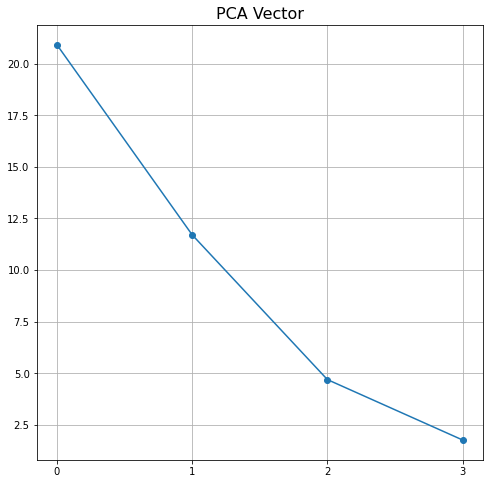
\includegraphics[width=0.51\textwidth]{fig/pcavec.png}
    \caption{PCA向量}
    &
    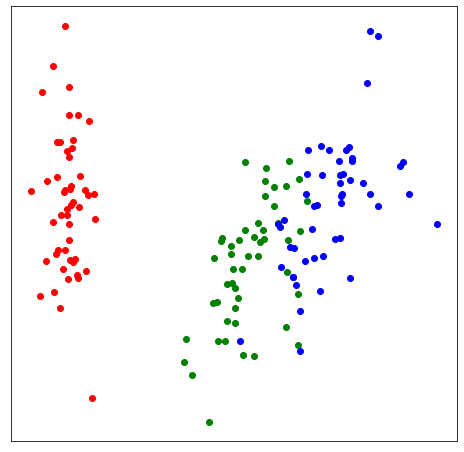
\includegraphics[width=0.49\textwidth]{fig/res.png}
    \caption{二维可视化}
    \end{tabular}
  \end{figure}

  \section{实验结果分析}
  从图1中可以看出,PCA向量的前两项具有比较大的值,说明其在特征空间中占据比较大的比重,
  因此可以只取前两项作为主要特征来对数据集进行分类。

  从图2中可以看出,使用PCA向量前两项作为x,y轴坐标,基本上可以把三类样本分开,因此使用
  PCA降维后依然能获得不错的分类效果
  \section{实验问题解答与体会}
  这次实验加深了我对PCA降维原理的理解,让我明白了并不是所有的样本数据都有必要参与训练。
  可以通过PCA来筛选出对结果影响比较大的特征进行训练,从而减少训练所需的运算量,提高训练速度,
  并且一定程度上能避免噪声的干扰

\end{document}
